\documentclass[../main.tex]{subfiles}

\begin{document}
\begin{enumerate}[(a)]

\item \textbf{(4 puntos)} Construya un histograma de frecuencias de las 35 empresas de acuerdo con el sector al que pertenece cada una. Muestre la tabla de frecuencias y la gráfica del histograma. ¿Cuáles son los 3 sectores de mayor frecuencia? ¿Qué porcentaje de la muestra es
representado por las empresas que pertenecen a estos sectores? ¿Cuáles son los sectores de menor frecuencia? ¿Qué porcentaje de la muestra es representado por las empresas que pertenecen a estos sectores?

\begin{figure}[h]
\centering
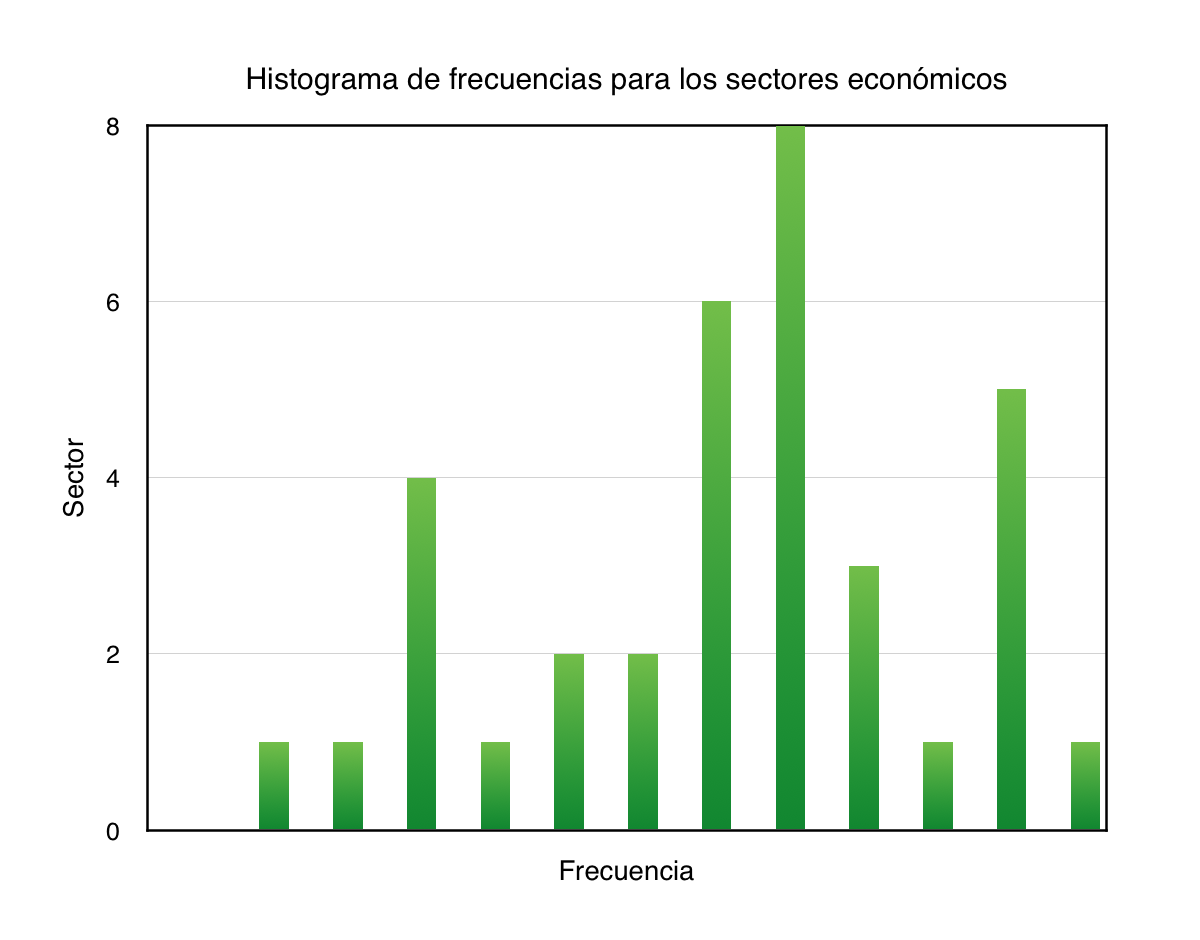
\includegraphics[width=10cm]{histo.png}
\label{fig:img1}
\end{figure}

Los sectores de mayor frecuencia son el financiero, el petrolero y el energético cada uno con 8, 5, y 6 empresas representativas. Cada una con 22.85\%, 14.28\% y 17.14\% respectivamente. Los sectores de menos frecuencia son  Aeronáutico, Aeronáutico, Comunicación, Comunicación y Textil. Cada uno con el 2.85\%.

\item \textbf{(4 puntos)} Construya un diagrama de caja que represente la distribución del precio promedio de la acción de las 35 empresas de la muestra. Comente sobre todos los elementos que representa el diagrama de caja.

\begin{figure}[h]
\centering
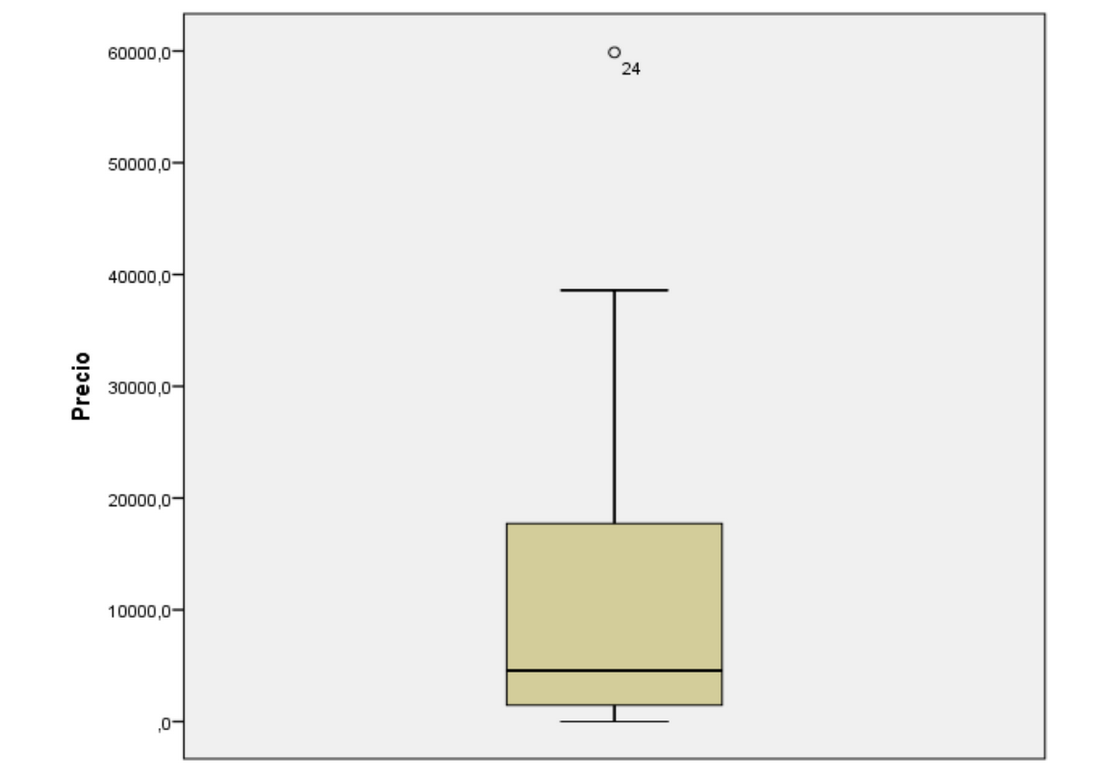
\includegraphics[width=10cm]{box.png}
\label{fig:img1}
\end{figure}

Se observa que la mayoría de los precios están sobre el delimitador de la caja.

\pagebreak

\item \textbf{(3 puntos)} Se desea analizar una nueva variable correspondiente al cociente entre el precio de la acción y los dividendos que promete ($P/D$). De acuerdo con este indicador se clasifica cada empresa de la siguiente manera:

\begin{figure}[h]
\centering
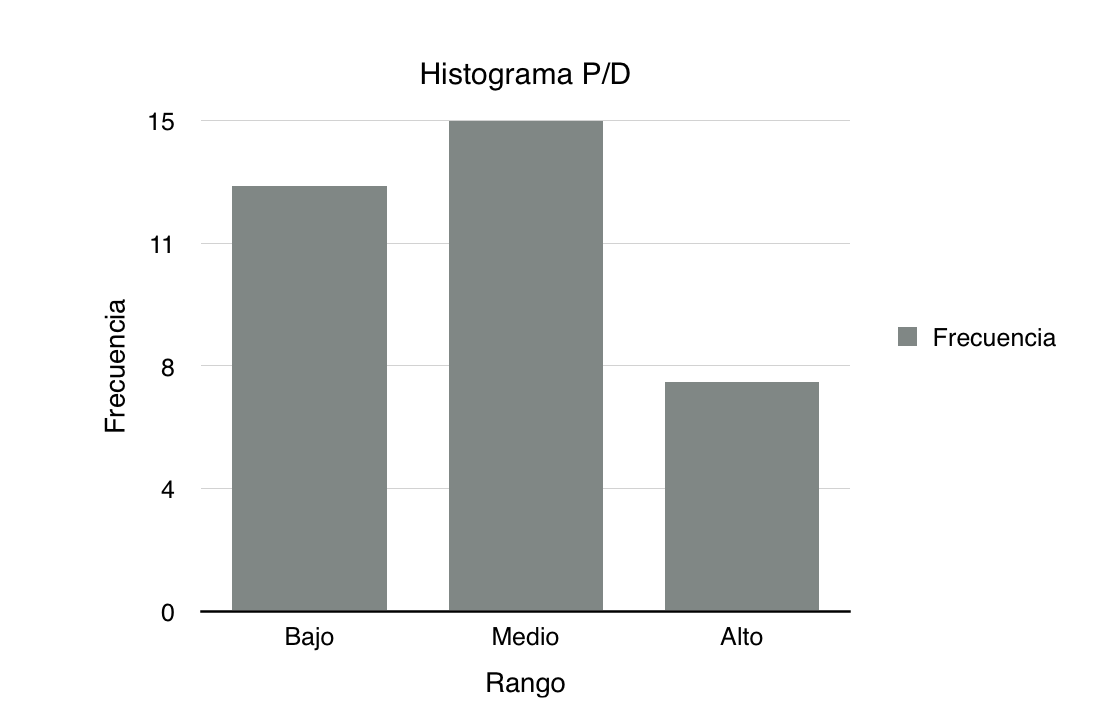
\includegraphics[width=8cm]{hist2.png}
\label{fig:img1}
\end{figure}

\pagebreak

\item \textbf{(2 puntos)} Los inversionistas están interesados en conocer cuáles son los tres sectores que prometen en promedio mayores dividendos. Para ello construya y presente una tabla dinámica que le permita comparar cada sector en términos de sus dividendos promedio.

\begin{figure}[h]
\centering
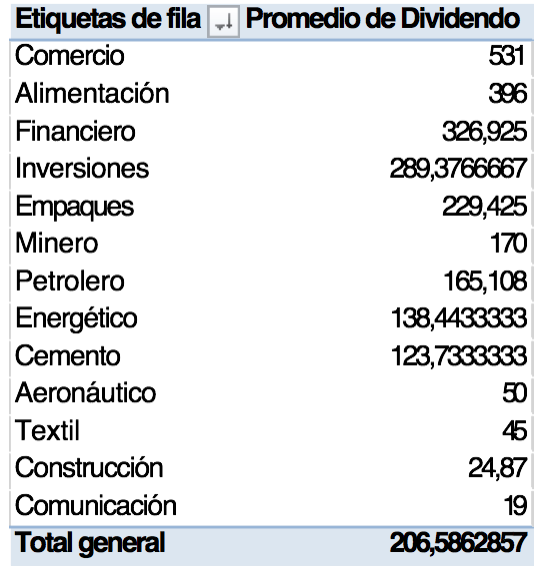
\includegraphics[width=6cm]{spss.png}
\label{fig:img1}
\end{figure}

\item \textbf{(2 puntos)} Los inversionistas han decidido establecer la siguiente clasificación partir de la ubicación de las empresas en el ranking Merco:

\item \textbf{(3 puntos)} Obtenga las estadísticas descriptivas de la variable precio/dividendo. ¿Qué puede concluir sobre la simetría y la curtosis de la distribución de los datos para la variable
precio/dividendo? ¿Cuál es la diferencia conceptual entre el error típico y la desviación
estándar?

\item \textbf{(4 puntos)} Presente la tabla de percentiles del precio promedio de las acciones.


\begin{figure}[h]
\centering
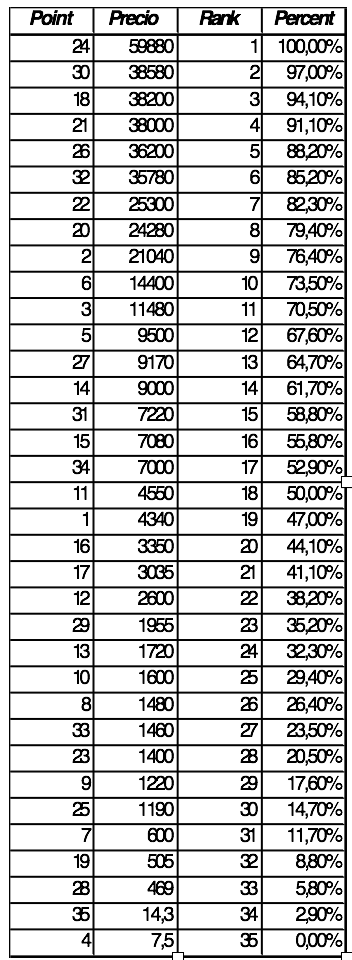
\includegraphics[width=6cm]{percent.png}
\label{fig:img1}
\end{figure}

\pagebreak

\begin{enumerate}[(I)]

\item ¿A qué compañía pertenece el percentil 50?

Cartón de Colombia. Ver gráfica al final

\item ¿Cuál es el precio de la acción y los dividendos asociados con esta compañía?

4500 COP y dividendos de 323.65' COP

\item ¿Cómo interpreta este resultado?
 Que este dato separa los datos en dos, es decir, e 50\% de los datos están arriba y los otros abajo

\end{enumerate}

\end{enumerate}
\end{document}
